\section{Ion Trap}

\section{Cryogenic Buffer Gas Beam}

The CBGB apparatus was homebuilt out of aluminum for the outer chamber as well as the inner 40K radiation shield. A Cryomech PT415 Pulse Tube Refrigerator with a remote head option was inserted into the chamber. A large bellows attachment connected the pulse tube cooler head to the chamber itself to isolate the chamber from the mechanical vibrations caused by the pulse tube cooler itself.

The pulse tube cooler itself has 2 cooling stages and a room temperature stage. The room temperature stage at the top is where 

\begin{figure}[H]
\centering
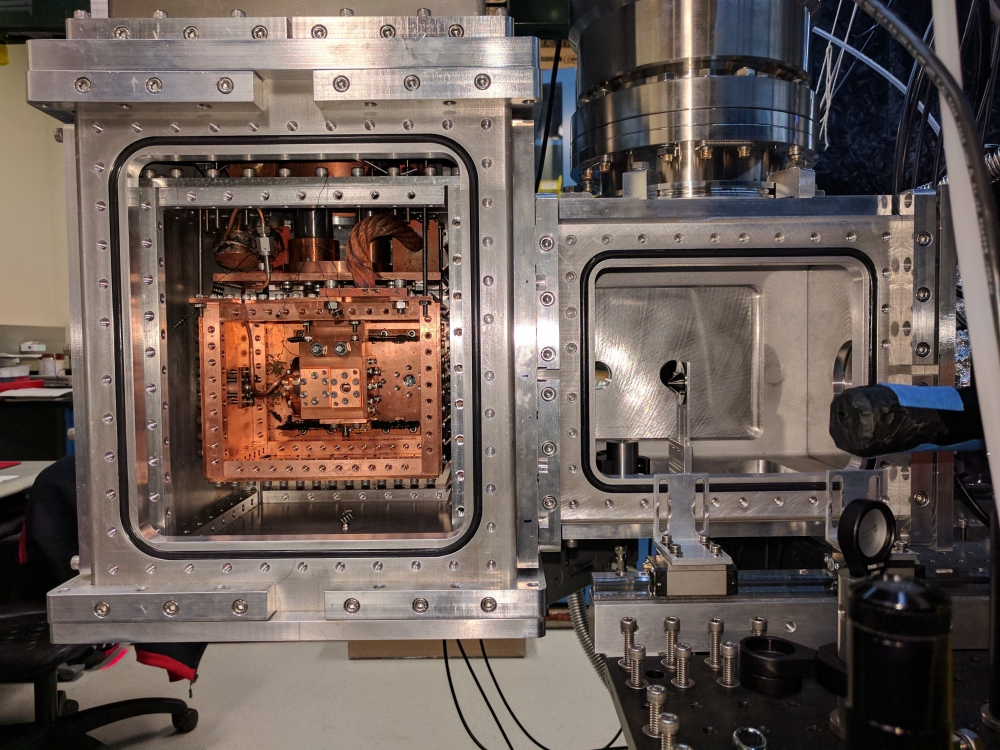
\includegraphics[width=1\textwidth]{images/apparatus_cross_section.jpg}
\caption{Cross sectional view of CBGB with side walls removed from the outer vacuum chamber, 40K aluminum radiation shield, and inner 4K cryopumping shield.}
\label{f: chamber}
\end{figure}

\begin{figure}[H]
\centering
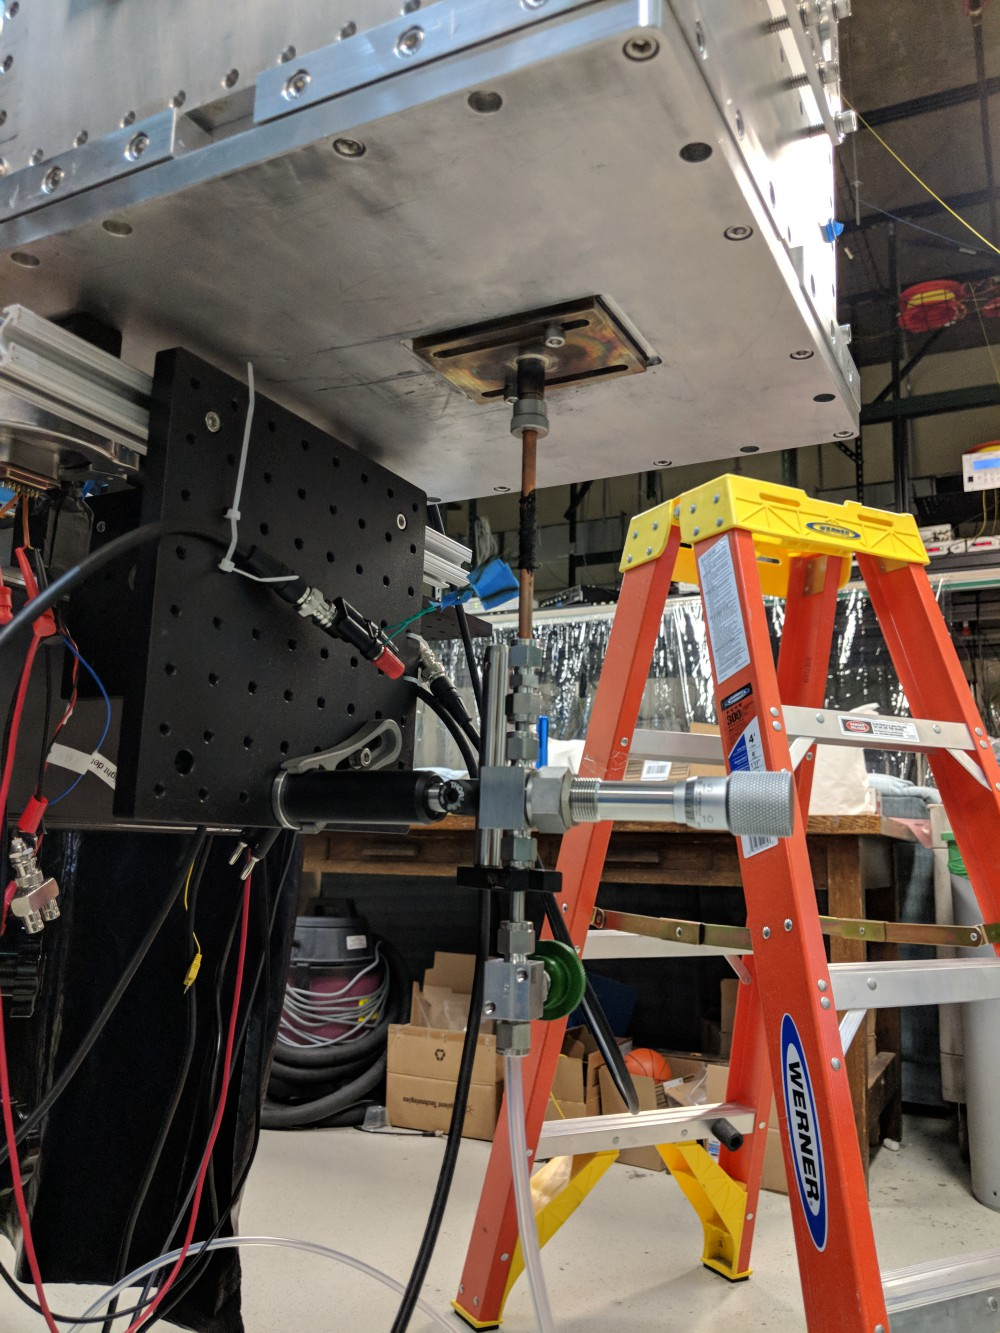
\includegraphics[width=.7\textwidth]{images/apparatus_water_fill_outside.jpg}
\caption{The water fill line, sealed by an ultratorr fitting and heated by nichrome wire. A shut off valve and vernier valve are used to regulate the flow of water into the buffer gas cell.}
\label{f: outside}
\end{figure}

\begin{figure}[H]
\centering
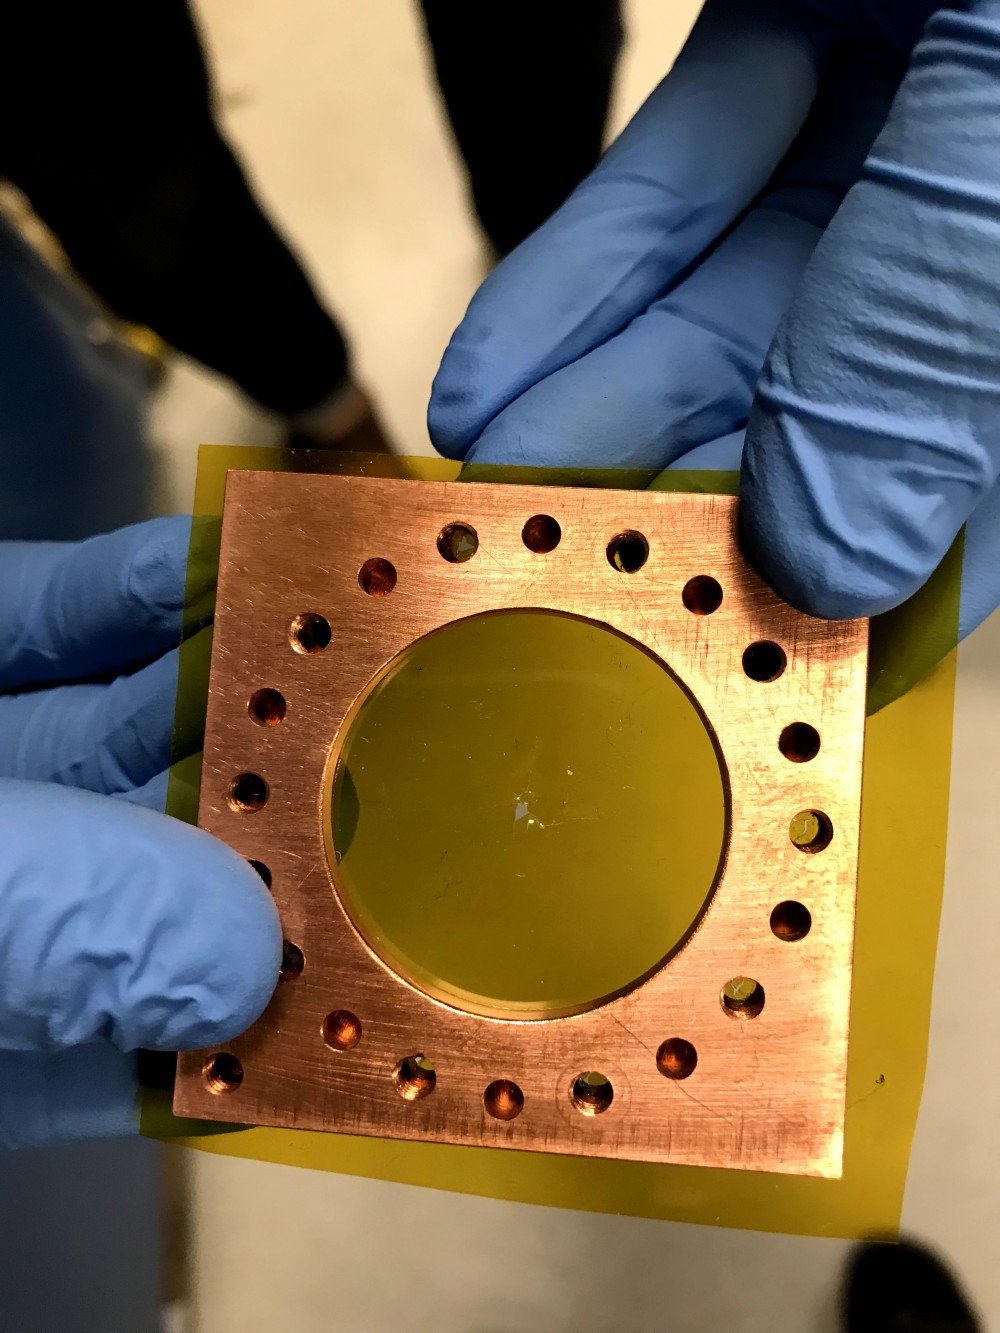
\includegraphics[width=.7\textwidth]{images/apparatus_kapton.jpg}
\caption{A kapton film serves as the back wall of the buffer gas cell with a hole for the insertion of the water fill line. The kapton surface resists ice formation and allows for continuous operation with water for over 10 hours.}
\label{f: kapton}
\end{figure}

\begin{figure} [H]
\centering
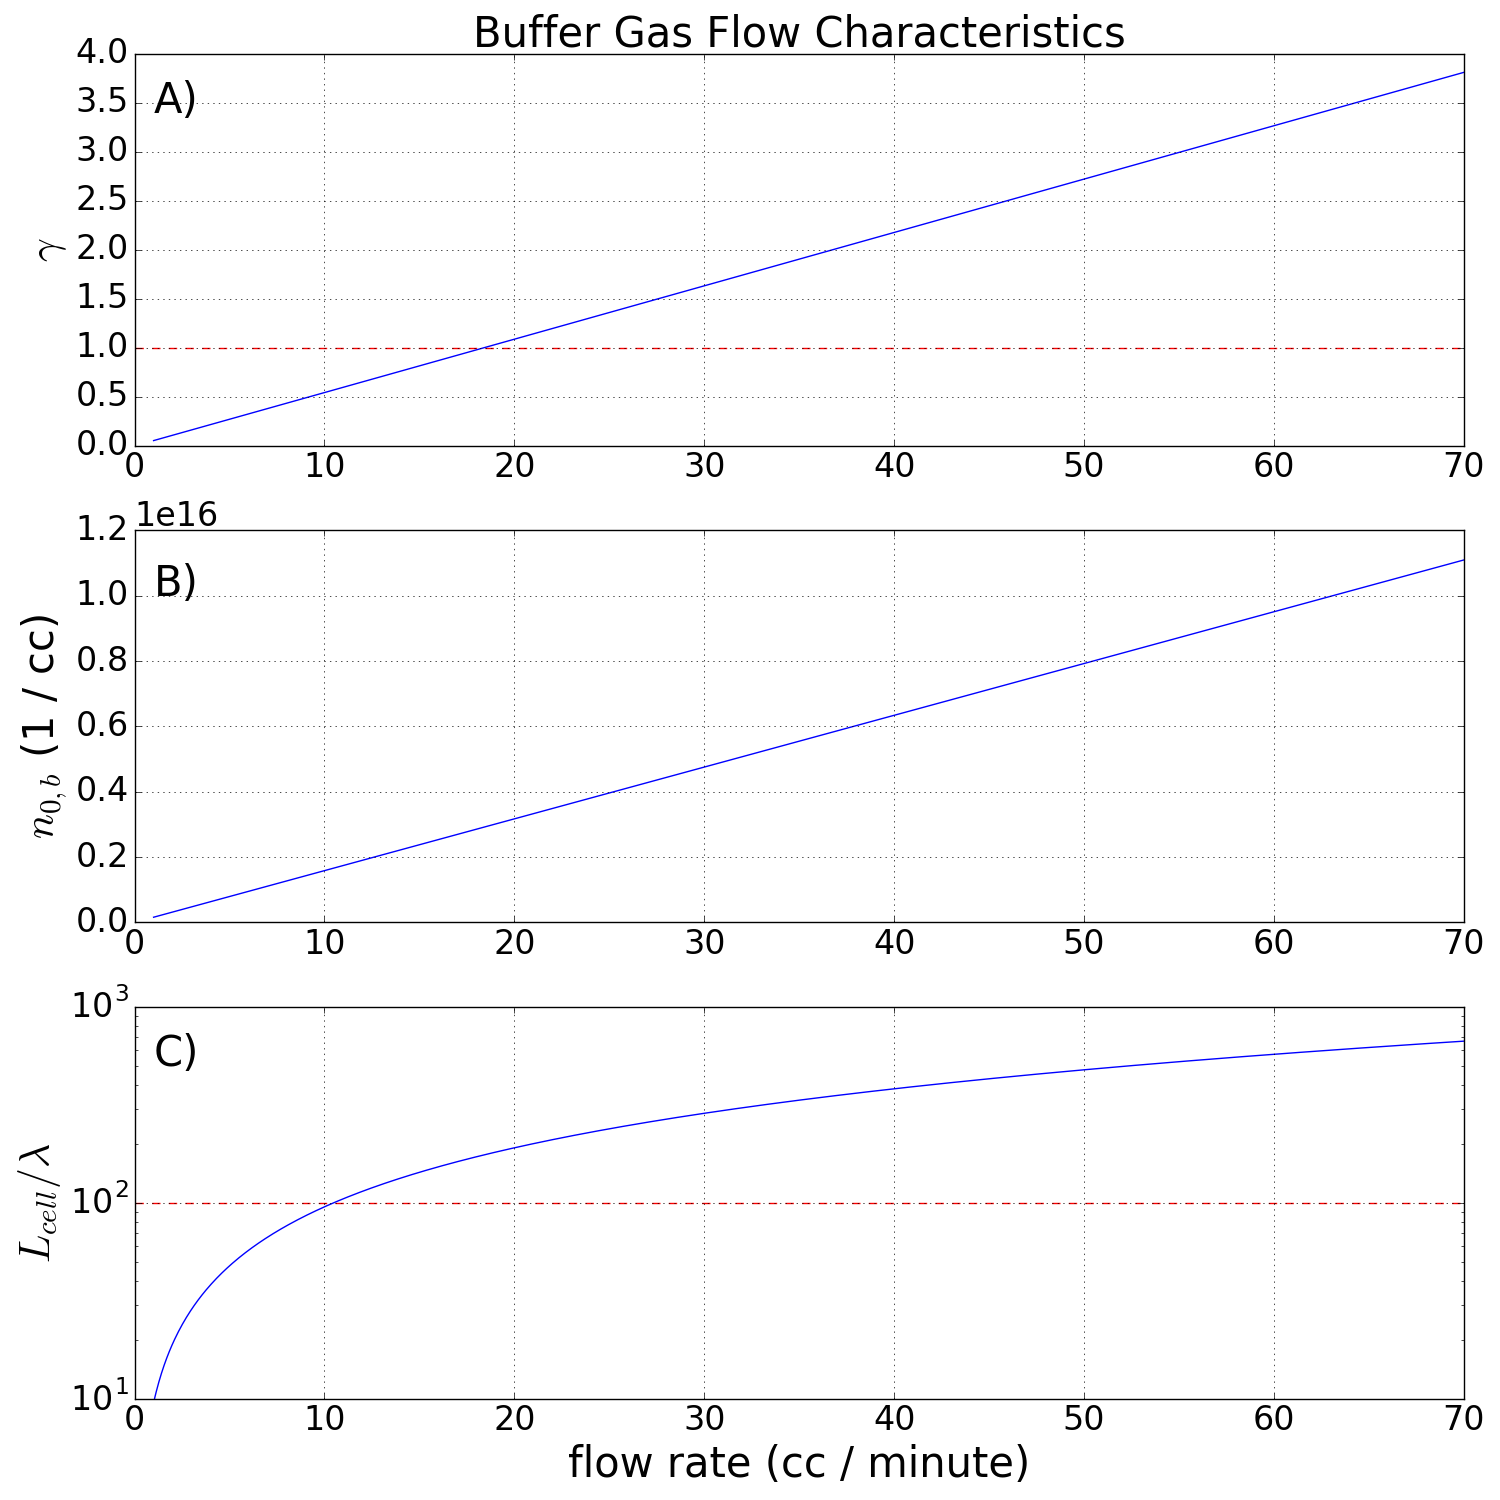
\includegraphics[width=1\textwidth]{images/CBGB_flow_characteristic.png}
\caption{A) $\gamma$ extraction ratio, dotted red line indicates $\gamma = 1$ where hydrodynamic entrainment begins. B) Theoretical number density of buffer gas species within buffer gas cell. C) Number of collisions one would expect before extraction out of the cell, dotted red line indicates 100 collisions before extraction when rotational degrees of freedom should be thermalized.}
\label{f: buffer_gas_flow}
\end{figure}

\subsection{Beam Density}

With our current capabilities, getting a good read on the beam density is difficult, we do not have a reliable method of characterizing the density at the trap region. We have utilized a residual gas analyzer (RGA) to determine the density of the beam in the ballistic regime upstream from the ion trap. Inserting the RGA into the beam path allows us to estimate the density of water in the beam as a function of the nominal buffer gas flow rate, as shown in figure \ref{f: rga}. Using that fit, we find good agreement with the theoretical calculations showing our flow to be near the supersonic regime, while staying in the hydrodynamic regime with a linear extraction efficiency dependence with the flow rate expressed in \ref{e: gamma}.

\begin{figure}[H]
\centering
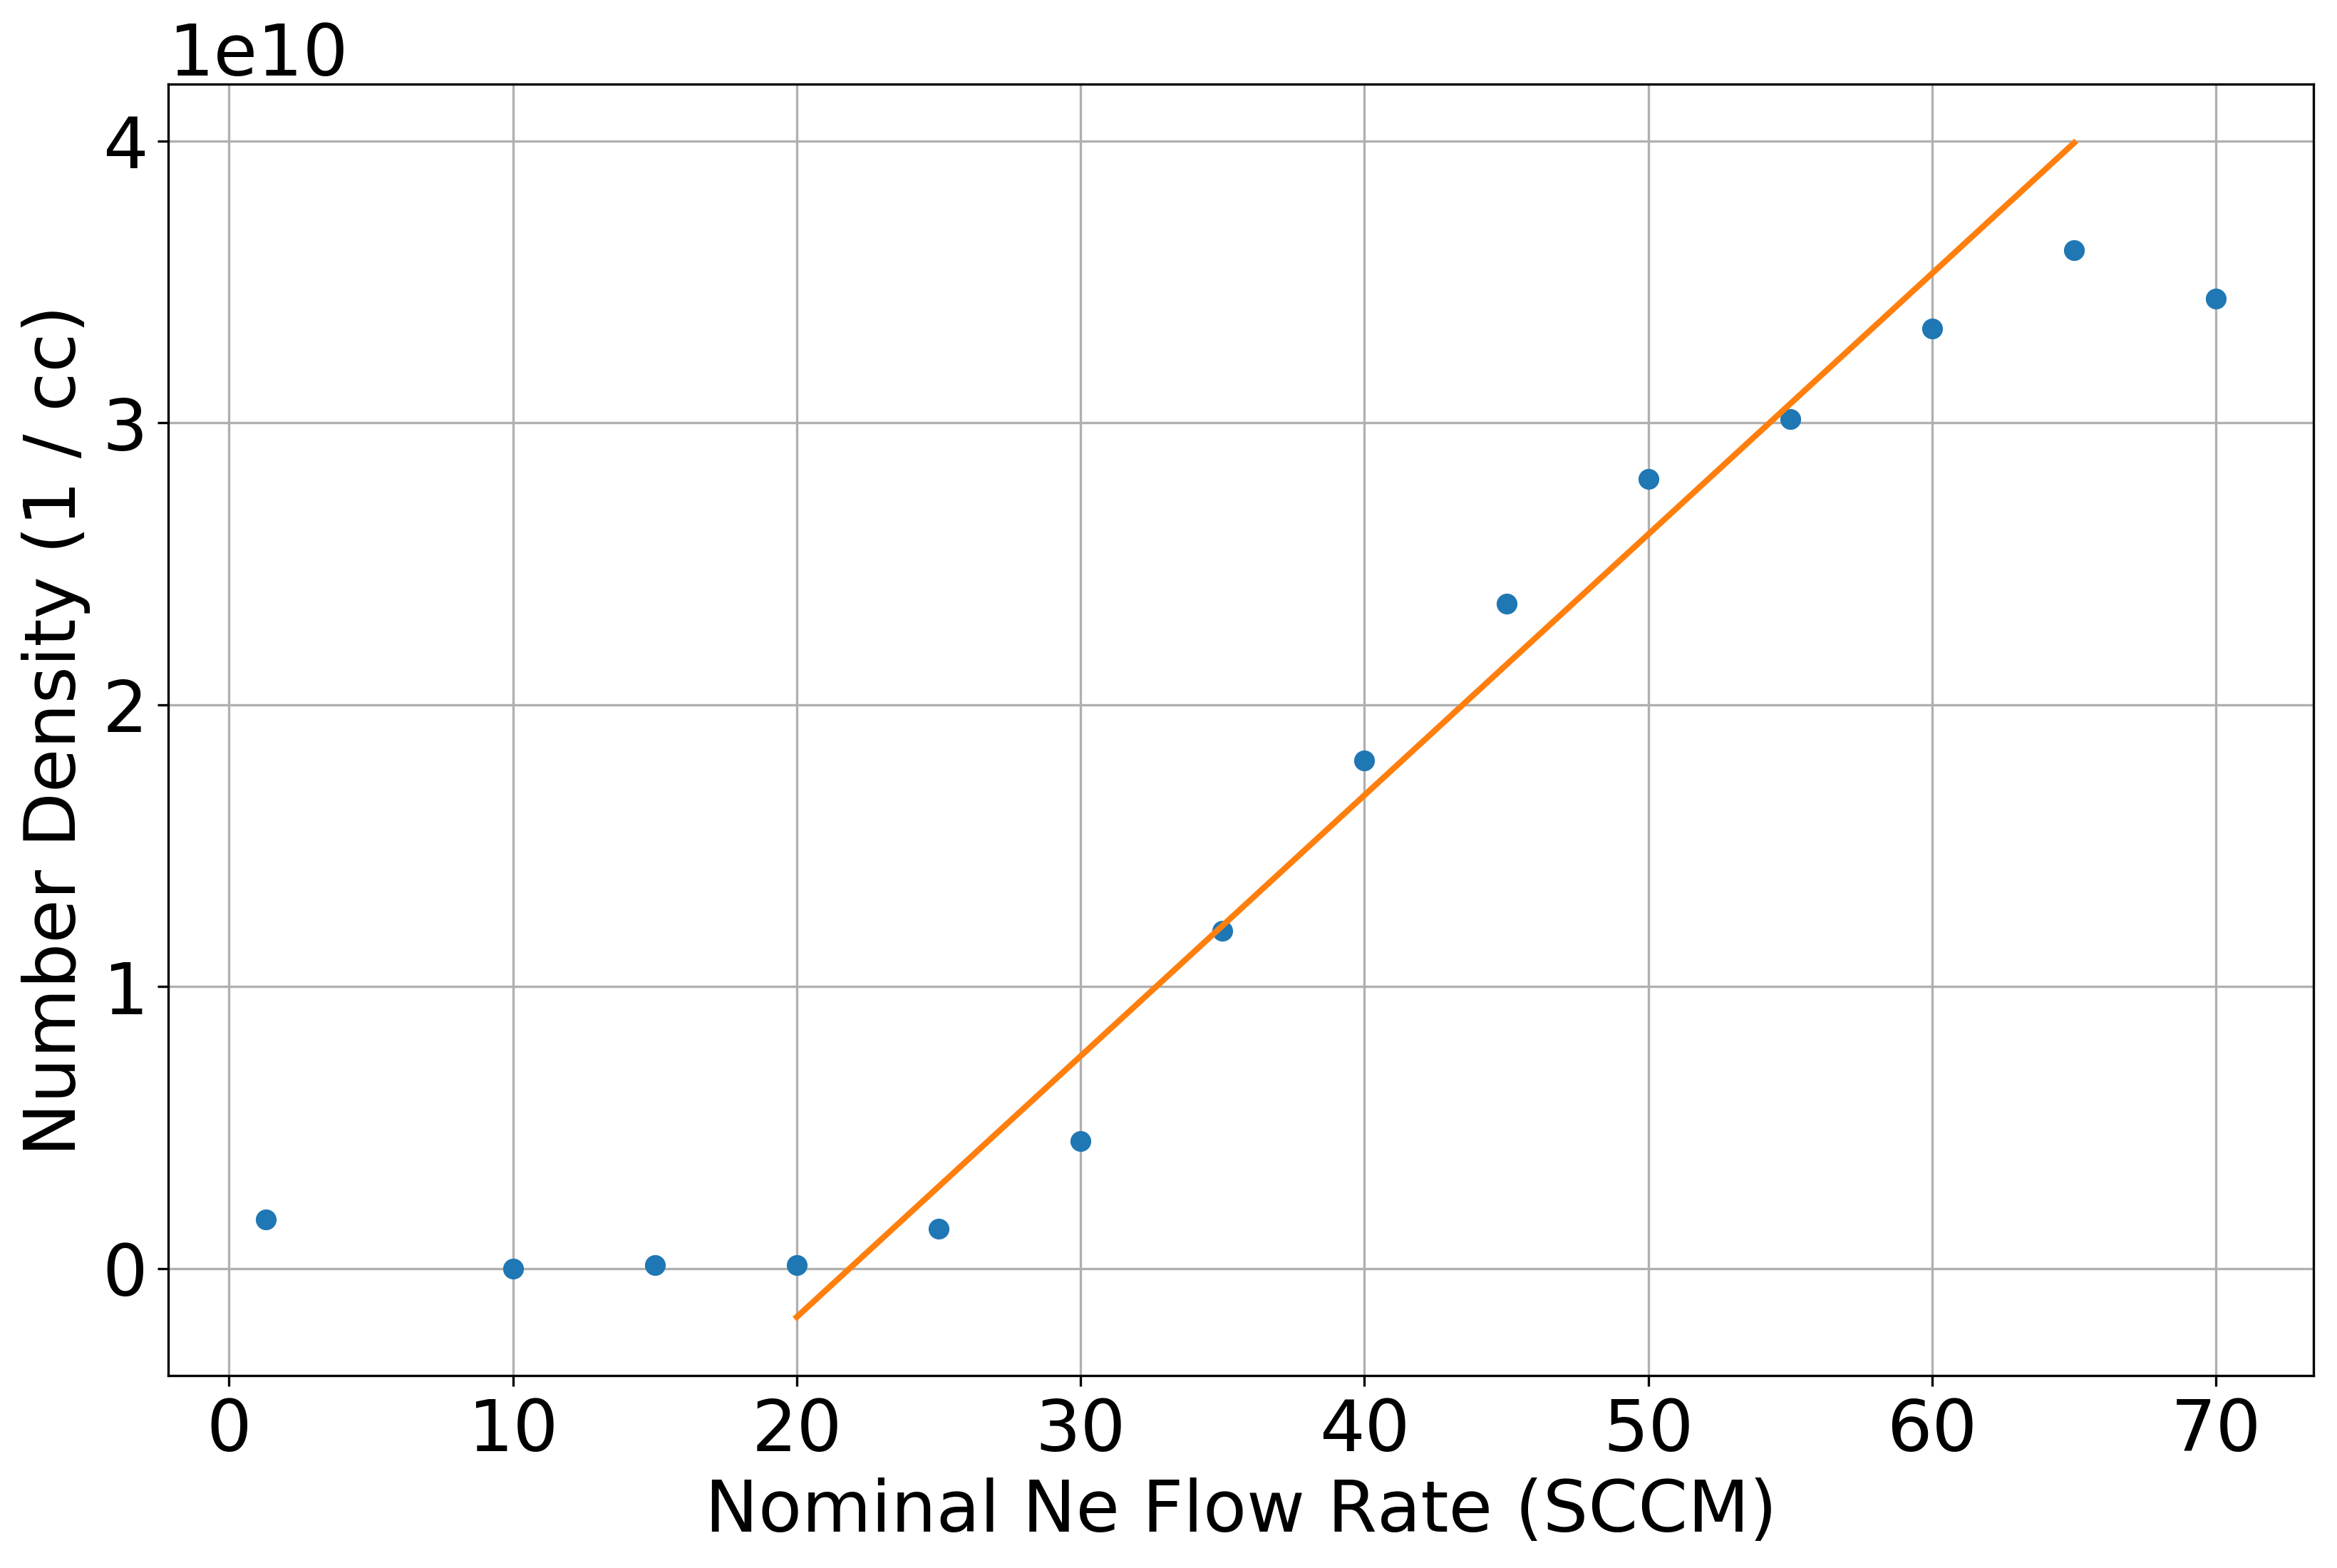
\includegraphics[width=1\textwidth]{images/CBGB_hydrodynamic_fit.png}
\caption{$1.12 \times 10^9 x + -2.75 \times 10^10$}
\label{f: rga}
\end{figure}

We know have previously calculated the possible number densities of the buffer gas with varying aperture sizes and flow rates. But now we can utilize those equations with the data on the target species to plot out the range of densities that we may see at the trap center as a function of the various apertures that we may utilize.

Knowing from our previous calculations:

$$ \bar{v} = \sqrt{\frac{8 k_B T}{m \pi}} $$
$$ n_{0,b}=\frac{4 f}{A_{aperture} \bar{v}} $$
$$n(z)=\frac{n_o}{2}\left(1-\frac{z}{\sqrt{z^2+a^2}}\right)$$

We can put it all together to get:

$$n(z)=\alpha\frac{f}{A_{aperture} \bar{v}}\left(1-\frac{z}{\sqrt{z^2+a^2}}\right)$$

But what we really care about is the region in which the number density is linearly dependent to the buffer gas flow rate, not over all possible ranges; we've seen that the target species only behaves linearly once it has been entrained in the buffer gas. This means that we should be equating the function of $n(z)$ with the linear fit performed on the data for the parameters the data was taken at.

$$mf+b = \alpha\frac{f}{A_{aperture, o} \bar{v_o}}\left(1-\frac{z_o}{\sqrt{z_o^2+a_o^2}}\right)$$

let

$$\beta = \frac{1}{A_{aperture, o} \bar{v_o}}\left(1-\frac{z_o}{\sqrt{z_o^2+a_o^2}}\right)$$

$$\alpha=\frac{m}{\beta}+\frac{b}{\beta f}$$

Thus, we may get a final form that incorporates the linear slope's dependence on the other variables of the system as well as the overall experimentally derived scaling factor from the data.

$$n(z)=\frac{mf+b}{A_{aperture} \bar{v} \beta}\left(1-\frac{z}{\sqrt{z^2+a^2}}\right)$$

There is a mass dependence in the thermal velocity equation, which leads us to conclude that the choice of the species is a statement of the effecacy of the beam itself. If we choose to calculate the thermal velocity of the target species found in the beam due to the theoretical thermal velocity of the buffer gas, that indicates that the beam properties are still dominated by the buffer gas species. This may not be the case, as we see in our data, we have a ratio of about 10:1, this is pushing the boundaries of the assumption that the buffer gas far outnumbers the target species. At these ratios, we may start to see the effects of the target species on the beam properties.

\begin{figure}[H]
\centering
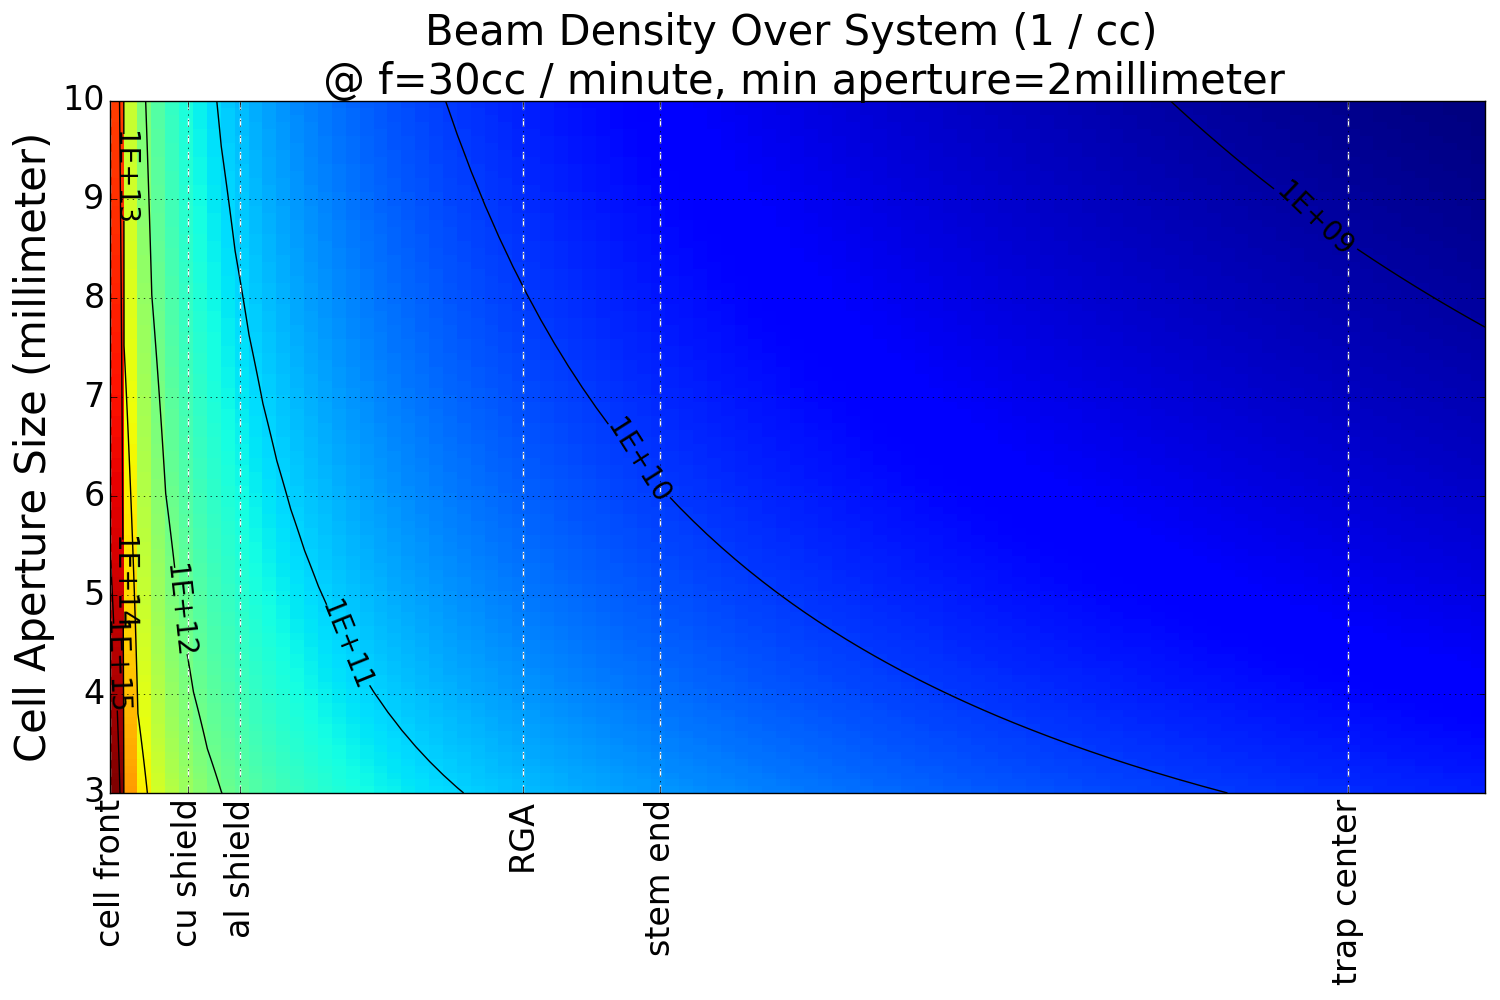
\includegraphics[width=1\textwidth]{images/CBGB_beam_density_over_system.png}
\caption{}
\label{f: beam_density}
\end{figure}

Extrapolating the fit and estimated density from figure \ref{f: rga}, we can estimate the density of the water at various locations along the beam line as shown in figure \ref{f: beam_density}. We find that we should be able to produce an appreciable number density of water down at the trap center.

From the RGA, we were able to open and close a shutter in the beam path and see an extinction of the water signal, but a more accurate representation would be from the ions in the trap themselves. We know that the trapped $Be^+$ ions will reaction with $H_2O$ to predominately produce $BeOH$, which we see as a drop in the fluorescence. Figure \ref{f: shutter_closing} shows fits of the fluorescence decay as a beam from the CBGB is suddenly blocked by our shutter in the beam line. Comparing the fitted reaction rates, we find that they agree with the background rates found as shown in figure \ref{f: shutter_bkg}. This indicates to us that we indeed have a beam of cryogenic water coming from the CBGB, as seen by the sudden extinction of the $Be^+ + H_2O$ reaction.

\begin{figure}[H] \label{f: shutter_bkg}
\centering
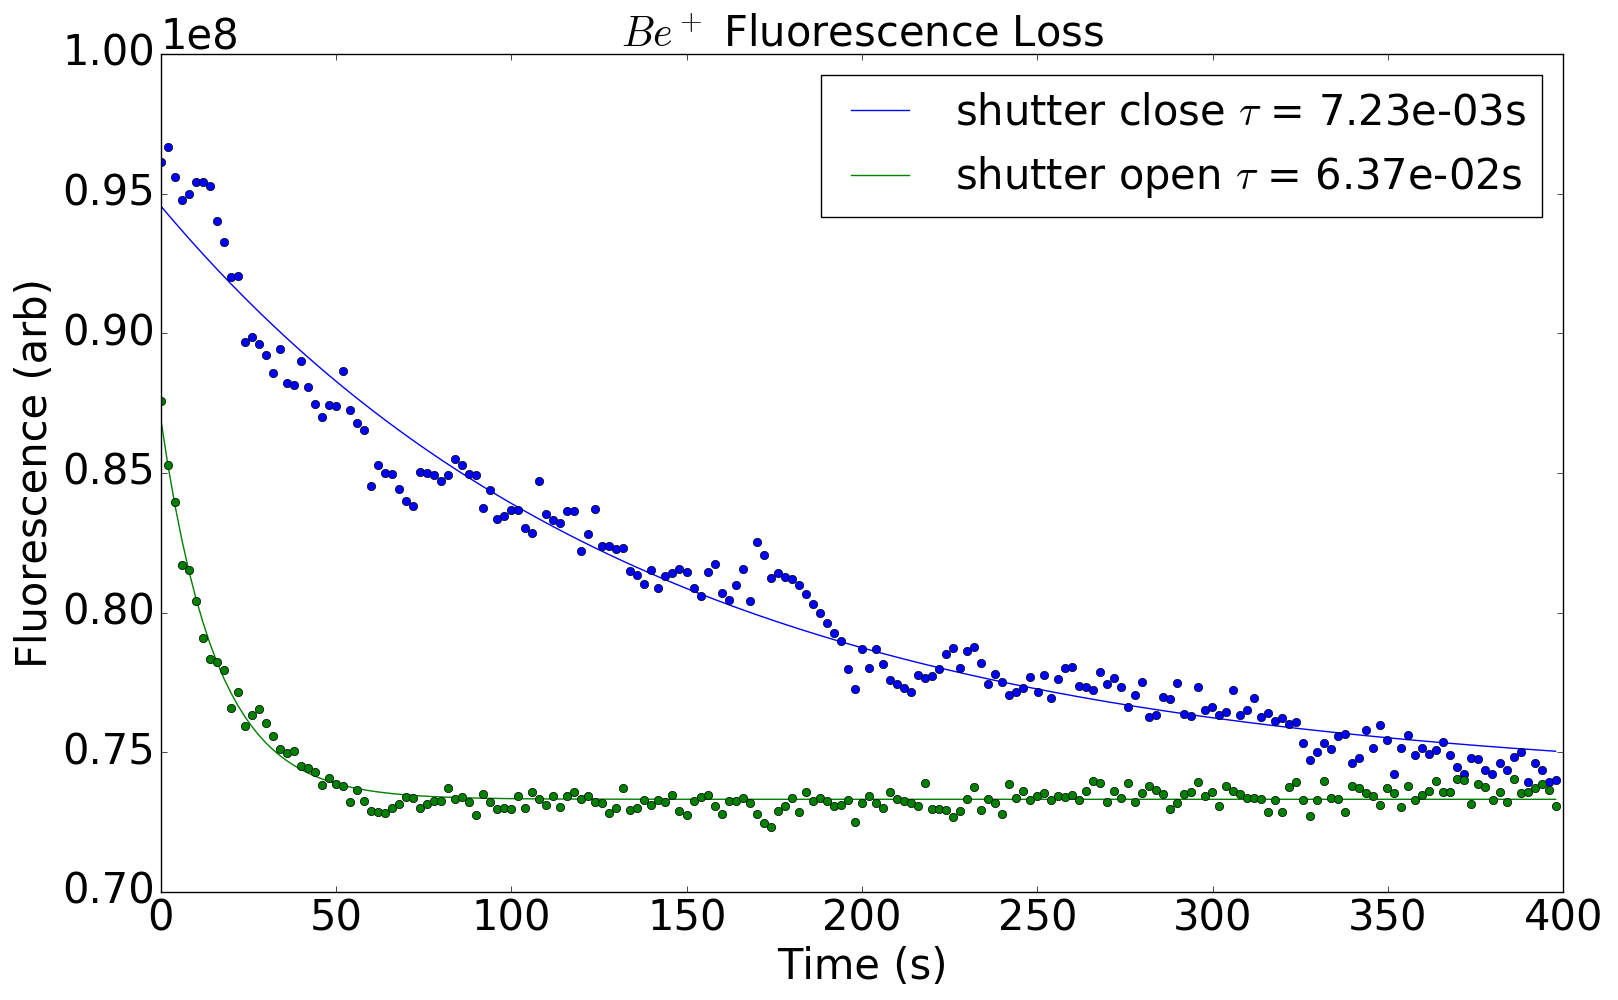
\includegraphics[width=1\textwidth]{images/CBGB_sudden_shutter_flow_bkg.png}
\caption{}
\end{figure}

\begin{figure}[H] \label{f: shutter_closing}
\centering
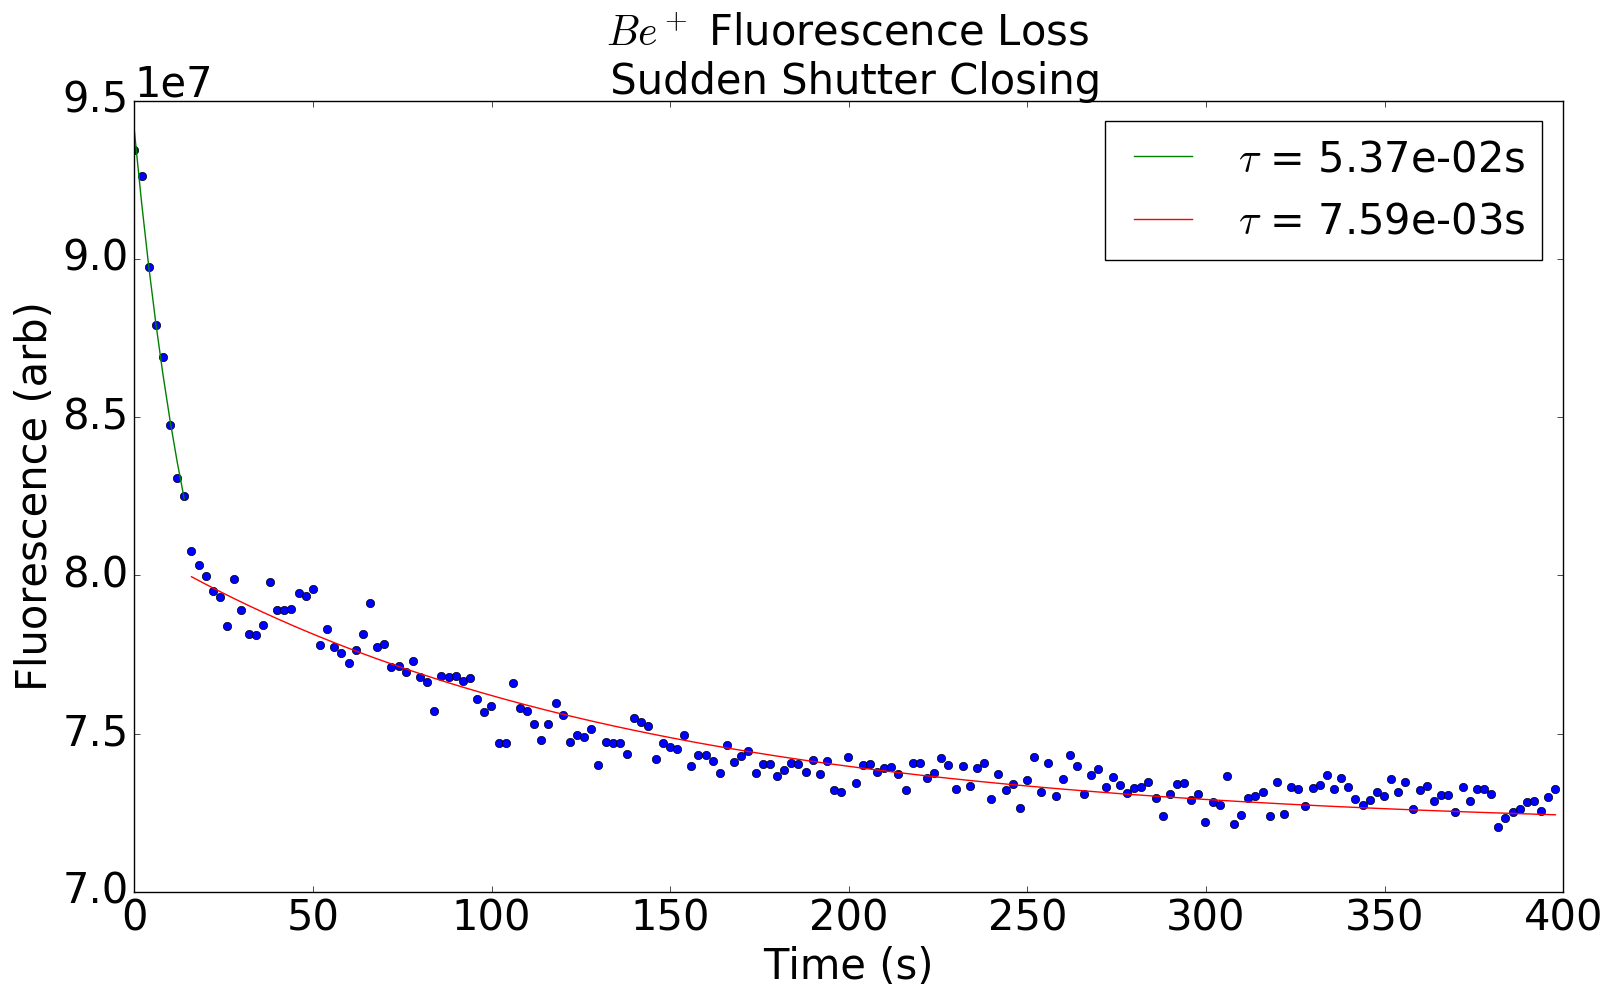
\includegraphics[width=1\textwidth]{images/CBGB_sudden_shutter_flow.png}
\caption{}
\end{figure}

\subsection{Beam Velocity}

To better understand the reaction temperatures we will be able to reach, we need a characterization of the beam's velocity, more specifically, the velocity of the target species entrained within the buffer gas. By ablating ytterbium into the neon buffer gas, we find that the ytterbium is entrained within the neon and sympathetically cooled to the cell's temperature. As long as the target species number density is a trace amount in comparison to the bulk buffer gas number density (1:1000), the flow characteristics are dominated by the buffer gas species \cite{Hutzler2012}. The forward velocity of the beam is not only parameterized by the temperature of the buffer gas species, it is also dependent on the flow regime. As we increase the flow of neon into the cell, figure \ref{f: rga} shows a linear increase in the $H_2O$ signal from a downstream RGA. This coincides with the beam operating within the intermediate flow regime, where there are few collisions at the cell aperture, resulting in a slight forward boosting and increased extraction efficiency of the target species. At higher flow regimes, entering the supersonic regime, we would see a "freeze out" where the forward velocity reaches $1.4\bar{v}$ and we would not see appreciable gains in species extraction \cite{Hutzler2012}. We chose to operate at a nominal neon flow rate of 30 sccm based upon the reaction rate of the ions downstream.

\begin{figure}[H]
\centering
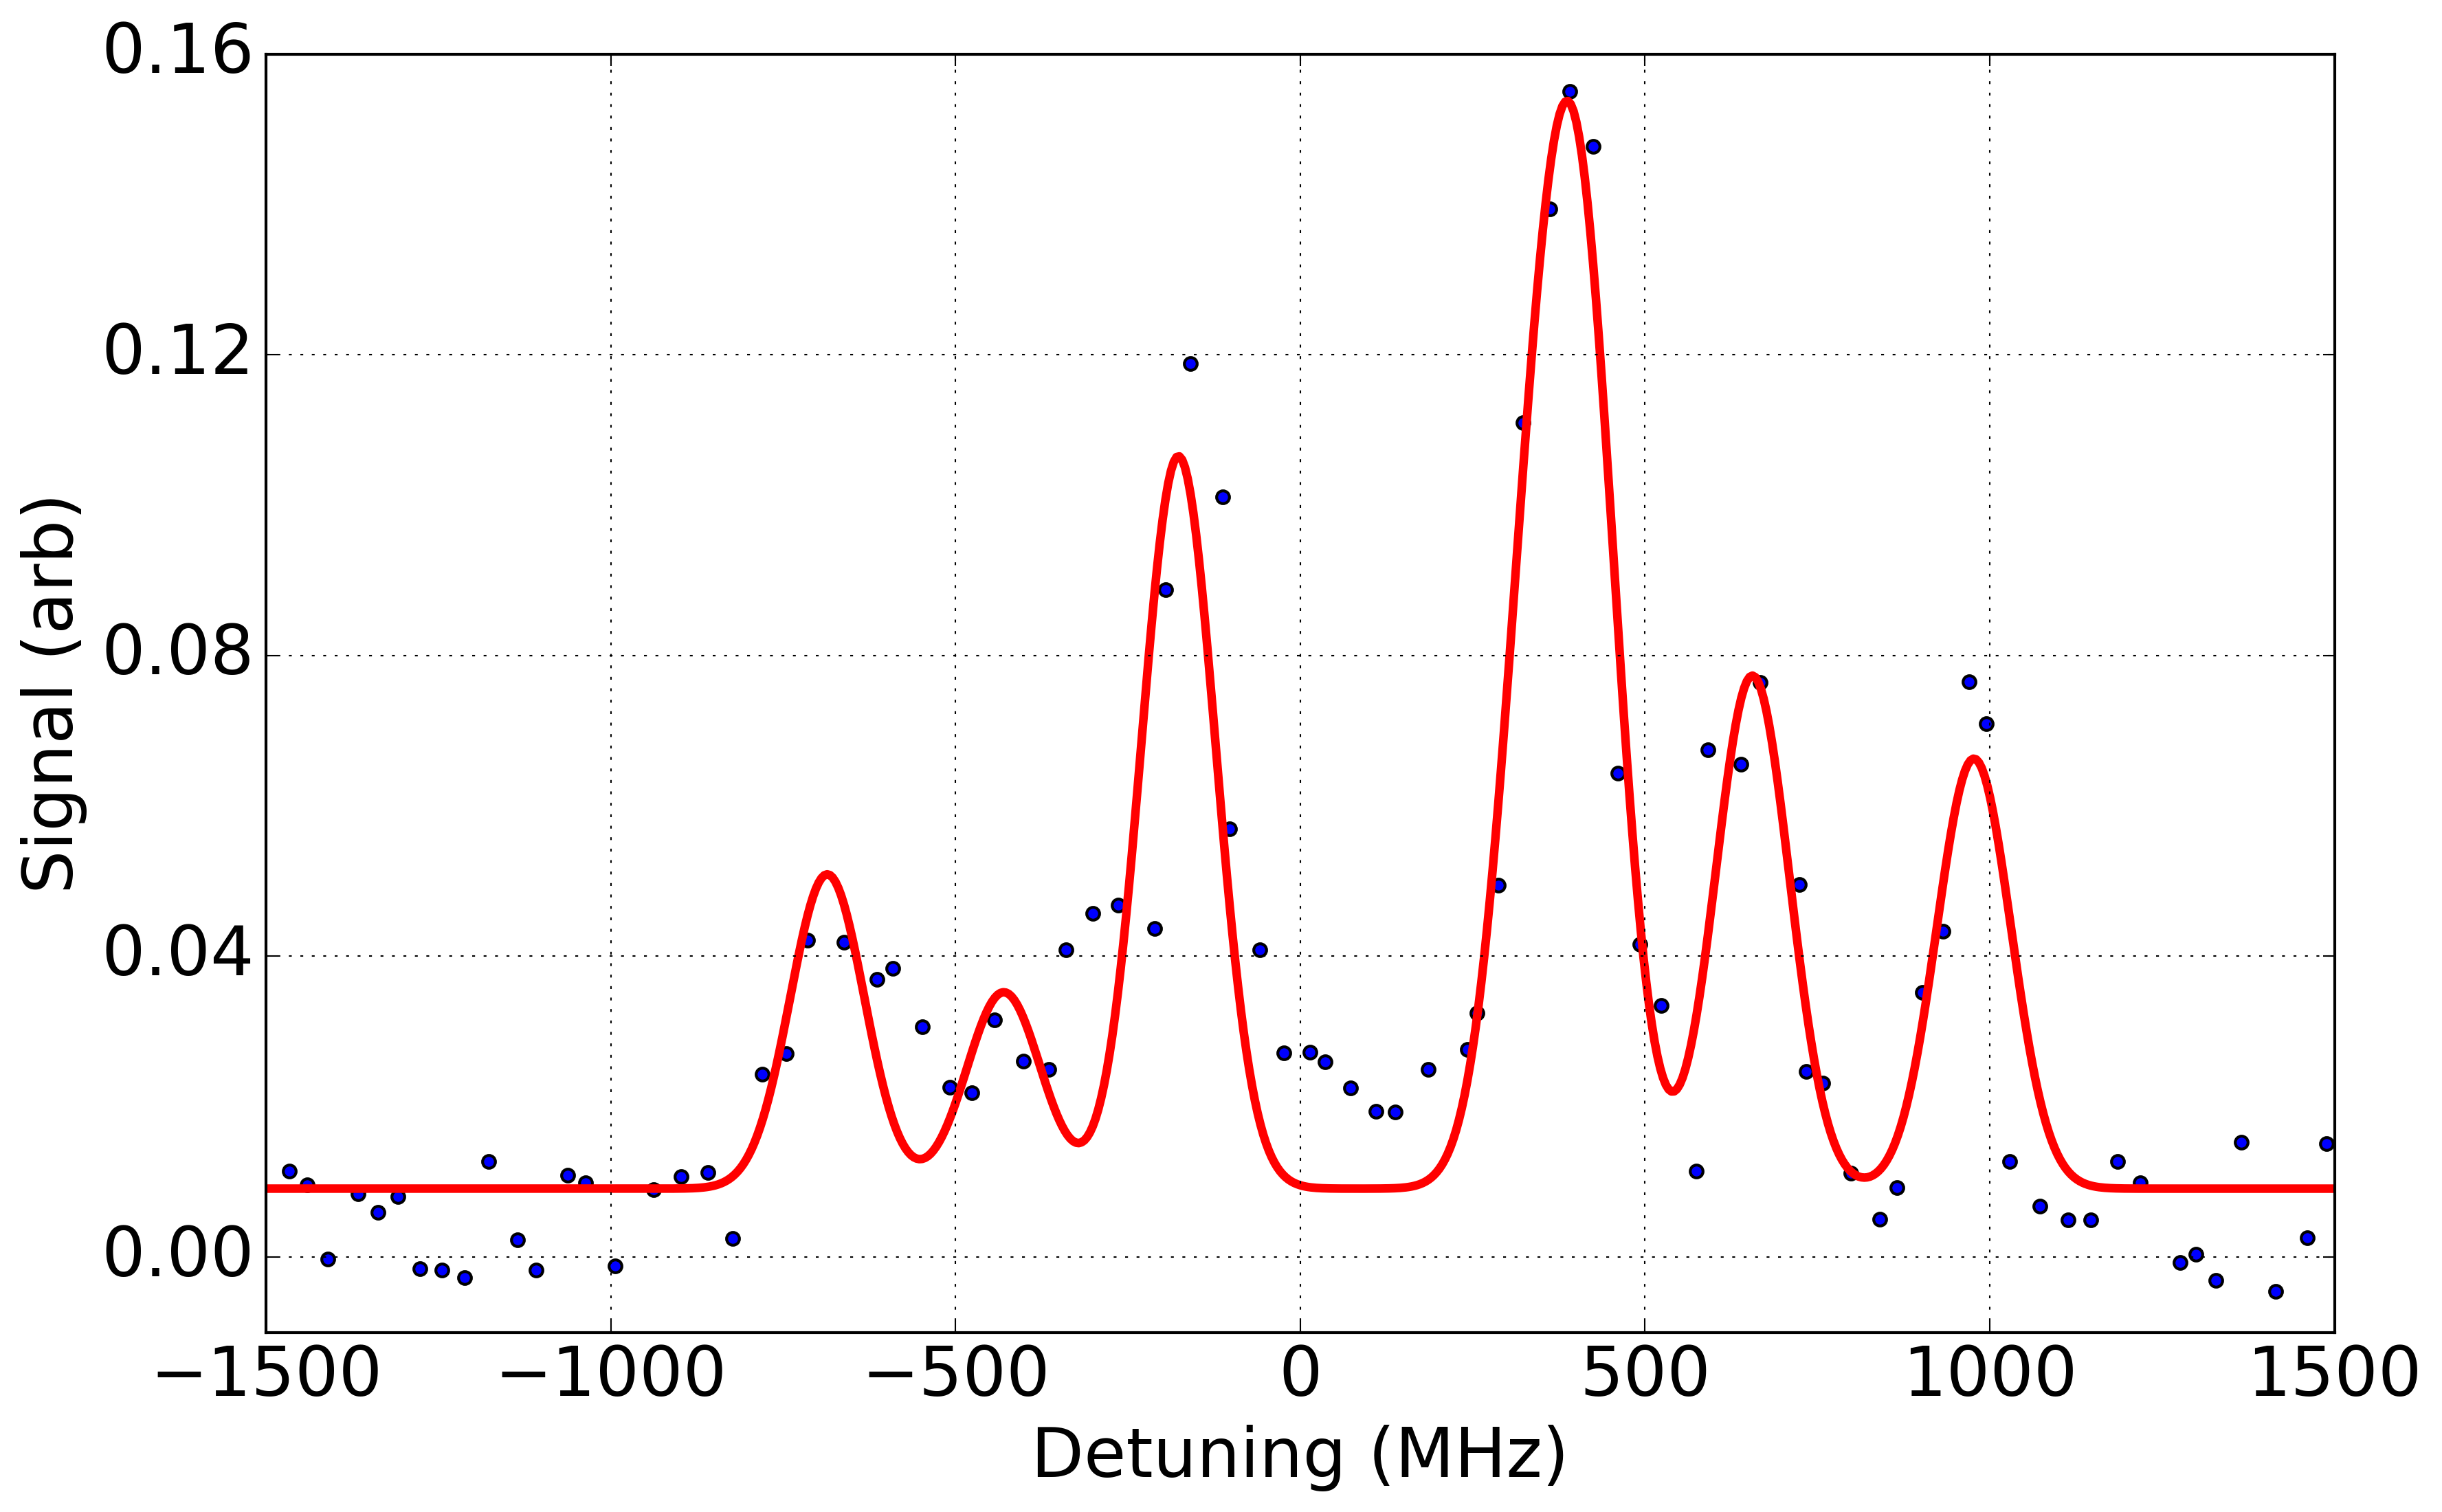
\includegraphics[width=1\textwidth]{images/CBGB_yb_spectrum_long.png}
\caption{\label{f: yb_spectrum}}
\end{figure}